% !TEX root = ../paper.tex
% This file was created with tikzplotlib v0.9.12.
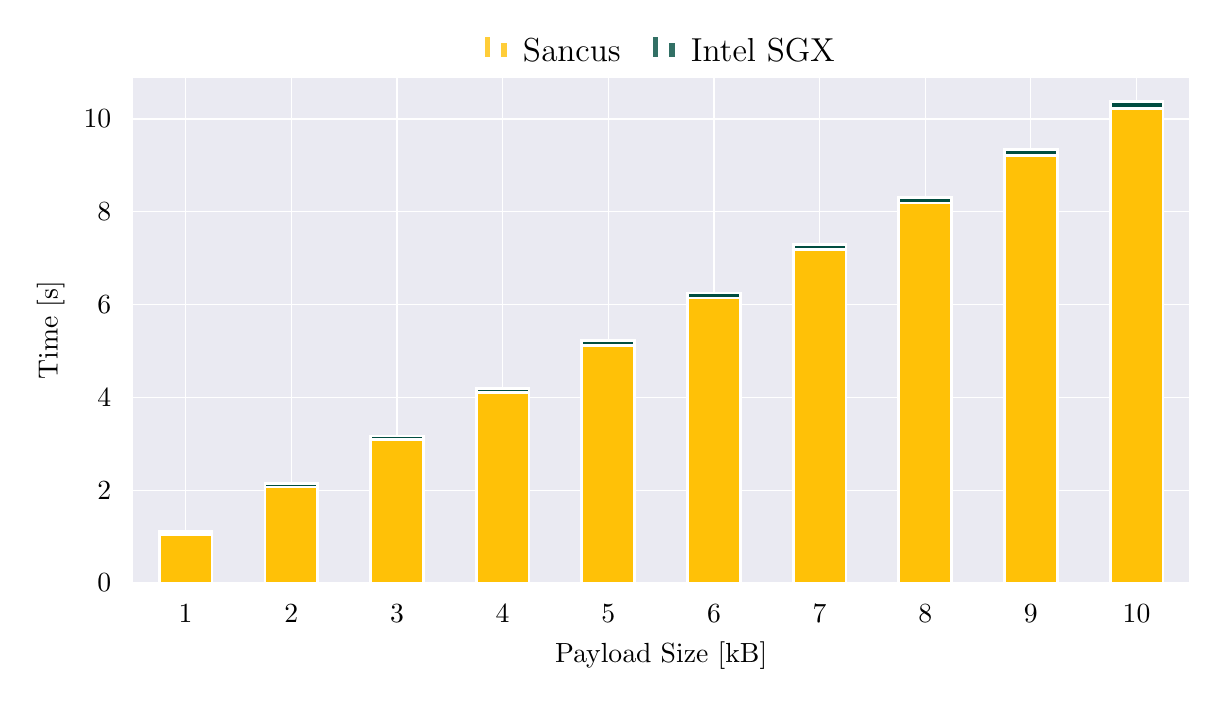
\begin{tikzpicture}

\definecolor{color0}{rgb}{0.917647058823529,0.917647058823529,0.949019607843137}
\definecolor{color1}{rgb}{1,0.756862745098039,0.0274509803921569}
\definecolor{color2}{rgb}{0,0.301960784313725,0.250980392156863}

\begin{axis}[
clip=false,
axis background/.style={fill=color0},
axis line style={white},
height=8cm,
legend cell align={left},
legend columns=2,
legend style={/tikz/every even column/.append style={column sep=0.3cm},/tikz/every odd column/.append style={column sep=0.1cm},font=\large,fill opacity=0.8, draw opacity=1, text opacity=1, at={(0.5,1)}, anchor=south, draw=none},
minor xtick={},
minor ytick={},
tick align=outside,
width=15cm,
x grid style={white},
xlabel={Payload Size [kB]},
xmajorgrids,
xmajorticks=true,
xmin=-0.5, xmax=9.5,
xtick style={color=white!15!black,draw=none},
xtick={0,1,2,3,4,5,6,7,8,9},
xticklabels={1,2,3,4,5,6,7,8,9,10},
y grid style={white},
ylabel={Time [s]},
ymajorgrids,
ymajorticks=true,
ymin=0, ymax=10.8925215,
ytick style={color=white!15!black,draw=none},
ytick={0,2,4,6,8,10,12}
]
\draw[draw=white,fill=color1,line width=1pt] (axis cs:-0.25,0) rectangle (axis cs:0.25,1.04712);
\addlegendimage{ybar,ybar legend,draw=white,fill=color1,line width=1pt}
\addlegendentry{Sancus}

\draw[draw=white,fill=color1,line width=1pt] (axis cs:0.75,0) rectangle (axis cs:1.25,2.06689);
\draw[draw=white,fill=color1,line width=1pt] (axis cs:1.75,0) rectangle (axis cs:2.25,3.08552);
\draw[draw=white,fill=color1,line width=1pt] (axis cs:2.75,0) rectangle (axis cs:3.25,4.1015);
\draw[draw=white,fill=color1,line width=1pt] (axis cs:3.75,0) rectangle (axis cs:4.25,5.12177);
\draw[draw=white,fill=color1,line width=1pt] (axis cs:4.75,0) rectangle (axis cs:5.25,6.13985);
\draw[draw=white,fill=color1,line width=1pt] (axis cs:5.75,0) rectangle (axis cs:6.25,7.18321);
\draw[draw=white,fill=color1,line width=1pt] (axis cs:6.75,0) rectangle (axis cs:7.25,8.18802);
\draw[draw=white,fill=color1,line width=1pt] (axis cs:7.75,0) rectangle (axis cs:8.25,9.20862);
\draw[draw=white,fill=color1,line width=1pt] (axis cs:8.75,0) rectangle (axis cs:9.25,10.22638);
\draw[draw=white,fill=color2,line width=1pt] (axis cs:-0.25,1.04712) rectangle (axis cs:0.25,1.10718);
\addlegendimage{ybar,ybar legend,draw=white,fill=color2,line width=1pt}
\addlegendentry{Intel SGX}

\draw[draw=white,fill=color2,line width=1pt] (axis cs:0.75,2.06689) rectangle (axis cs:1.25,2.13674);
\draw[draw=white,fill=color2,line width=1pt] (axis cs:1.75,3.08552) rectangle (axis cs:2.25,3.16622);
\draw[draw=white,fill=color2,line width=1pt] (axis cs:2.75,4.1015) rectangle (axis cs:3.25,4.19129);
\draw[draw=white,fill=color2,line width=1pt] (axis cs:3.75,5.12177) rectangle (axis cs:4.25,5.22197);
\draw[draw=white,fill=color2,line width=1pt] (axis cs:4.75,6.13985) rectangle (axis cs:5.25,6.25039);
\draw[draw=white,fill=color2,line width=1pt] (axis cs:5.75,7.18321) rectangle (axis cs:6.25,7.30108);
\draw[draw=white,fill=color2,line width=1pt] (axis cs:6.75,8.18802) rectangle (axis cs:7.25,8.31572);
\draw[draw=white,fill=color2,line width=1pt] (axis cs:7.75,9.20862) rectangle (axis cs:8.25,9.34621);
\draw[draw=white,fill=color2,line width=1pt] (axis cs:8.75,10.22638) rectangle (axis cs:9.25,10.37383);
\end{axis}

\end{tikzpicture}
